\section{Phenotype}
\label{methodology_phenotype}

In order to test the quality of maps and have something that potentially could be put into the StarCraft II Editor, a structure that can represent the entire map is required. We refer to it as the phenotype, again the word used in genetic algorithms.

As mentioned above, a map is made up of height-levels and various features the players can use to their advantage. In a map it is possible for a a single cell to contain a height-level (it always will), a location for a base\footnote{We save the centre locations of bases for use with the fitness function.} and destructible rocks that have to be cleared before a base can be built. This situation require three $n$-by-$m$ grids in order to properly represent:

\begin{my_itemize}

	\item The first grid represents the heightmap. It has the following states: Impassable terrain, height 0, height 1, height 2, ramp, or cliff.

	\item The second grid represents the actual position of different map features; Bases, minerals, gas, and xel'naga towers.

	\item The third grid represents where destructible rocks are positioned in the map.

\end{my_itemize}

\subsection{Functionality of the Structure}
\label{methodology_phenotype_functionality}

Generation of the \textit{initial heightmap} and \textit{smoothing of the heightmap}\footnote{Both generation and smoothing are only focused on height-levels, not on cliffs or ramps. The placement of cliffs are handled by the map structure and placement of ramps is handled by the phenotype.} are both handled by a cellular automata (see section \ref{methodology_ca}) and will not be discussed in-depth here.

\subsubsection*{Cliff Placement}

\textit{Placement of cliffs} is a straight-forward process. In StarCraft, cliffs form the natural border between two height-levels (see figure \ref{fig:Editor_CliffExample}). We find, and create, the cliffs by iterating over all tiles in the heightmap and finding every tile's neighbours (using the von Neumann neighbourhood, see figure \ref{fig:CA_Neighbourhoods} on page \pageref{fig:CA_Neighbourhoods}). If any neighbour is of a lower level, that neighbour is changed to become a cliff\footnote{Unless something is in the way, such as minerals, gas, or xel'naga towers.}. In the event that a tile has two or more neighbours of lower level, that tile is a corner of that section of height-level. The tile, and its neighbours, are changed to cliffs, as that is how StarCraft represents the corner of a height-level (as see in figure \ref{fig:Editor_CliffExample}).

\insertPicture{0.8}{Editor_CliffExample}{A section of cliffs in the StarCraft map editor. Notice how the corner of the cliff appears to be on the higher level.}{Editor_CliffExample}

\subsubsection{Cliff Smoothing}

After cliffs have been placed, it is possible that cliffs have been placed in such a way that they do not border up to form a border between height-levels. This can happen in situations where one of the two height-levels only take up a small area. After placing cliffs, we iterate over the heightmap once more. If a cliff is found, its neighbours are checked (this time using Moore neighbourhood) and if it does not have two different height-levels in its neighbourhood, the cliff is changed to whatever height-level it bordered up to. 

During the smoothing process, if any tile is found that is only connected to one other tile of the same height-level\footnote{This is checked using the von Neumann neighbourhood.}, that tile is transformed into a cliff and the position is saved. For every saved position, the area in a 3-by-3 square around it is run through the smoothing process again. This may seem counterintuitive, but in StarCraft the minimum size of a height-level area is 2-by-2. Any height-level tile \textbf{must} therefore have at least two other tiles next to it, otherwise it is not a valid height.

\subsubsection{Visual Representation}
When a map has been fully created (that means after the representation has been converted, see section \ref{methodology_conversion}), a visual representation can be created. Every state in the heightmap, the feature map and the rock map has a picture of a tile mapped to it. These tiles are draws on a bitmap, in the order of heightmap, features and rocks. This map is saved to a PNG file which can be opened and analyzed. For an example of the visual representation, see figure \ref{fig:methodology_genotype_differentbasemaps} on page \pageref{fig:methodology_genotype_differentbasemaps}.

A legend of the different tiles can be seen here:

\begin{my_itemize}

	\item 
\includegraphics[scale=0.7]{Images/Tiles/Height0} - Height level 0.

	\item 
\includegraphics[scale=0.7]{Images/Tiles/Height1} - Height level 1.

	\item 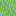
\includegraphics[scale=0.7]{Images/Tiles/Height2} - Height level 2.

	\item 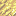
\includegraphics[scale=0.7]{Images/Tiles/Cliff} - A cliff between height levels.

	\item 
\includegraphics[scale=0.7]{Images/Tiles/Ramp01} \& 
\includegraphics[scale=0.7]{Images/Tiles/Ramp12} - Ramps between height levels.

	\item 
\includegraphics[scale=0.7]{Images/Tiles/Impassable} - Impassable terrain.

	\item 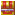
\includegraphics[scale=0.7]{Images/Tiles/StartBase} - The area a start base is supposed to cover.

	\item 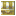
\includegraphics[scale=0.7]{Images/Tiles/Base} - The area intended for the base for an expansion.

	\item 
\includegraphics[scale=0.7]{Images/Tiles/BlueMinerals} \& 
\includegraphics[scale=0.7]{Images/Tiles/GoldMinerals} - The two types of minerals, blue and gold respectively.

	\item 
\includegraphics[scale=0.7]{Images/Tiles/Gas} - The area covered by a gas depot.

	\item 
\includegraphics[scale=0.7]{Images/Tiles/XelNaga} - The placement of a Xel'Naga tower.

	\item 
\includegraphics[scale=0.7]{Images/Tiles/DestructibleRocks} - An area covered by destructible rocks.

\end{my_itemize}